\begin{figure}[H]
    \centering
    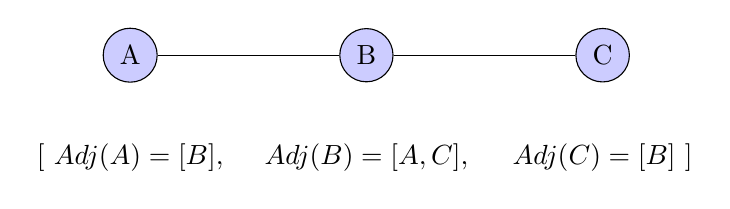
\begin{tikzpicture}
        \node[circle, draw, fill=blue!20] (A) at (0,0) {A};
        \node[align=center, below] at (0, -1) {[ $Adj(A)=[B]$,};
        \node[circle, draw, fill=blue!20] (B) at (3,0) {B};
        \node[align=center, below] at (3, -1) {$Adj(B)=[A,C]$,};
        \node[circle, draw, fill=blue!20] (C) at (6,0) {C};
        \node[align=center, below] at (6, -1) {$Adj(C)=[B]$ ]};
        \draw (A) -- (B);
        \draw (B) -- (C);
    \end{tikzpicture}
    \caption{Adjacency List representation for an undirected graph.}
    \label{fig:adjacency-list-undirected}
\end{figure}